%%%%%%%%%%%%%%%%%%%%%%%%%%%%%%%%%%%%%%%%%%%%%%%%%%%%%%%%%%%%%%%%%%%%
%
%   Style for CMS Computing / Physics Technical Design Reports
%
%   Lucas Taylor  4 Feb 2005,   Revised  12 Oct 2005
%
%%%%%%%%%%%%%%%%%%%%%%%%%%%%%%%%%%%%%%%%%%%%%%%%%%%%%%%%%%%%%%%%%%%%

%  the following line is edited by the tdr script to change or to pass
%  additional options:
\documentclass{cmspaper}
\usepackage{slashed}
\usepackage{subfigure}
%\usepackage{rotating}
\usepackage{multirow}
\usepackage{amsmath}
\usepackage{graphicx}
\usepackage{units}
\setkeys{Gin}{width=\linewidth,totalheight=\textheight,keepaspectratio}
\graphicspath{{fig/}}

%\usepackage{amsmath}
%\usepackage{bm}
%\usepackage{float}
%\usepackage{axodraw}
%\usepackage{sparticles} 	%Package for displaying sparticle names. 
%\usepackage{feynmf}		%Package for feynman diagrams. 
\def\centeron#1#2{{\setbox0=\hbox{#1}\setbox1=\hbox{#2}\ifdim
\wd1>\wd0\kern.5\wd1\kern-.5\wd0\fi
\copy0\kern-.5\wd0\kern-.5\wd1\copy1\ifdim\wd0>\wd1
\kern.5\wd0\kern-.5\wd1\fi}}
\def\ltap{\;\centeron{\raise.35ex\hbox{$<$}}{\lower.65ex\hbox{$\sim$}}\;}
\def\gtap{\;\centeron{\raise.35ex\hbox{$>$}}{\lower.65ex\hbox{$\sim$}}\;}
\def\gsim{\mathrel{\gtap}}
\def\lsim{\mathrel{\ltap}}

%%%%%%%%%%%%%%%%%%%%%%%%%%%%%%%%%%%%%%%%%%%%%%%%%%%%%%%%%%%%%%%%%%%%

%
% My Macros
%
\usepackage{graphicx}
%\usepackage{drftcite}
\usepackage{pstricks}
\usepackage[figuresright]{rotating}
%
%
% Macro declarations
%
%---- SLASH
\def\slasha#1{#1\hskip-0.65em /}  %slasha per caratteri piccoli
\def\slashb#1{#1\hskip-1.3em /}   %slashb per quelli grandi
\def\slashc#1{#1\hskip-.4em /}
%
%---- UNITA` DI MISURA
\def \pb        {{\rm \, pb}}
\def \fb        {{\rm \, fb}}
\def \ipb       {{\rm \, pb^{-1}}}
\def \ifb       {{\rm \, fb^{-1}}}
\def \eV        {{\rm \,  eV}}
\def \keV       {{\rm \, keV}}
\def \MeV       {{\rm \, MeV}}
\def \GeV       {{\rm \, GeV}}
\def \TeV       {{\rm \, TeV}}
\def \TeVc      {\TeV/c}
\def \TeVcc     {\TeV/c^2}
\def \GeVc      {\GeV/c}
\def \GeVcc     {\GeV/c^2}
\def \MeVc      {\MeV/c}
\def \MeVcc     {\MeV/c^2}
%
%---- SIMBOLI
\def\ga{\mathrel{\raise.3ex\hbox{$>$\kern-.75em\lower1ex\hbox{$\sim$}}}}
\def\la{\mathrel{\raise.3ex\hbox{$<$\kern-.75em\lower1ex\hbox{$\sim$}}}}
\newcommand {\lesssim}
     {\,\raisebox{-0.6ex}{$\stackrel{\textstyle<}{\textstyle\sim}$}\,}
\newcommand {\gtrsim}
     {\,\raisebox{-0.6ex}{$\stackrel{\textstyle>}{\textstyle\sim}$}\,}
\newcommand{\ckm}{$\checkmark$}
%
%---- MISCELLANEA
%\newcommand {\slashed}[1] { \mbox{\rlap{\hbox{/}} #1 }}
\newcommand {\onehalf}    {\raisebox{0.1ex}{${\frac{1}{2}}$}}
\newcommand {\fivethirds} {\raisebox{0.1ex}{${\frac{5}{3}}$}}
\newcommand {\OR}         {{\tt OR}\,}
\newcommand {\BR}         {{\rm BR}\,}
\newcommand {\rts}        {\sqrt{s}}
\newcommand {\lumi}       {\mathcal{L}}
\newcommand {\Lumi}       {\int\lumi\mathrm{d}t}
\newcommand {\gradi}    {^\circ}
\newcommand {\de}         {\partial}
\newcommand {\um}         {\, \mu \rm m}
\newcommand {\nm}         {\rm \, nm}
\newcommand {\us}         {\, \mu \rm s}
\newcommand {\cm}         {\rm \, cm}
\newcommand {\mm}         {\rm \, mm}
\newcommand {\m}          {\rm \, m}
\newcommand {\km}         {\rm \, km}
\newcommand {\V}          {\rm \, V}
\newcommand {\T}          {\rm \, T}
\newcommand {\kV}         {\rm \, kV}
\newcommand {\kVm}        {\rm \, kV\! / \! m} 
\newcommand {\MVm}        {\rm \, MV\! / \! m} 
\newcommand {\ns}         {\rm \, ns} 
\newcommand {\ps}         {\rm \, ps} 
%
%---- THEORY groups & AOB
\newcommand {\gws}        {\mathrm{SU(2)_L \otimes U(1)_Y}}
\newcommand {\sul}        {\mathrm{SU(2)_L}}
\newcommand {\suc}        {\mathrm{SU(3)_C}}
\newcommand {\ul}         {\mathrm{U(1)_Y}}
\newcommand {\uem}        {\mathrm{U(1)_{em}}}
\newcommand {\sigmabar}   {\overline{\sigma}}
\newcommand {\gmunu}      {g^{\mu \nu}}
\newcommand {\munu}       {{\mu \nu}}
\newcommand {\obra}       {\langle 0 |}
\newcommand {\oket}       {| 0 \rangle}
%
%---- THEORY lepton fields
\newcommand {\LL}         {L^{\alpha}_{\mathrm L}}
\newcommand {\LLd}        {L^{\dagger \alpha}_{\mathrm L}}
\newcommand {\lL}         {\ell^{\alpha}_{\mathrm L}}
\newcommand {\lLd}        {\ell^{\dagger \alpha}_{\mathrm L}}
\newcommand {\ld}         {\ell^{\dagger \alpha}}
\newcommand {\lb}         {\overline{\ell}^{\alpha}}
\newcommand {\lR}         {\ell^{\alpha}_{\mathrm R}}
\newcommand {\lRd}        {\ell^{\dagger \alpha}_{\mathrm R}}
\newcommand {\nuL}        {\nu^{\alpha}_{\mathrm L}}
\newcommand {\nuLb}       {\overline{\nu}^{\alpha}_{\mathrm L}}
\newcommand {\nub}        {\overline{\nu}^{\alpha}}
\newcommand {\lept}       {\ell^\alpha}
\newcommand {\neut}       {\nu^{\alpha}}
\newcommand {\nuLd}       {\nu^{\dagger \alpha}_{\mathrm L}}
\newcommand {\Phid}       {\Phi^\dagger}
%
%---- THEORY quark fields
\newcommand {\up}         {u^{\alpha}}
\newcommand {\ub}         {\overline{u}^{\alpha}}
\newcommand {\down}       {d^{\alpha}}
\newcommand {\db}         {\overline{d}^{\alpha}}
\newcommand {\QL}         {Q^{\alpha}_{\mathrm L}}
\newcommand {\QLd}        {Q^{\dagger \alpha}_{\mathrm L}}
\newcommand {\UL}         {U^{\alpha}_{\mathrm L}}
\newcommand {\ULd}        {U^{\dagger \alpha}_{\mathrm L}}
\newcommand {\UR}         {U^{\alpha}_{\mathrm R}}
\newcommand {\URd}        {U^{\dagger \alpha}_{\mathrm R}}
\newcommand {\DL}         {D^{\alpha}_{\mathrm L}}
\newcommand {\DLd}        {D^{\dagger \alpha}_{\mathrm L}}
\newcommand {\DR}         {D^{\alpha}_{\mathrm R}}
\newcommand {\DRd}        {D^{\dagger \alpha}_{\mathrm R}}
\newcommand {\bfell}      {\ell\kern-0.4em
                           \ell\kern-0.4em
                           \ell\kern-0.4em
                           \ell }
\newcommand {\obfell}     {\overline{\ell}\kern-0.4em
                           \overline{\ell}\kern-0.4em
                           \overline{\ell}\kern-0.4em
                           \overline{\ell}}
\newcommand {\bfH}      {\, {\cal H}\kern-0.5em \kern-0.4em
                           {\cal H}\kern-0.5em \kern-0.4em
                           {\cal H}\kern0.1em }
\newcommand {\obfH}     {\, \overline{\cal H}\kern-0.5em \kern-0.4em 
                           \overline{\cal H}\kern-0.5em \kern-0.4em 
                           \overline{\cal H}\kern0.1em }
%
%---- PARTICELLE
\def \b             {{\mathrm b}}
\def \t             {{\mathrm t}}
\def \charm         {{\mathrm c}}
\def \d             {{\mathrm d}}
\def \u             {{\mathrm u}}
\def \e             {{\mathrm e}}
\def \q             {{\mathrm q}}
\def \g             {{\mathrm g}}
\def \p             {{\mathrm p}}
\def \s             {{\mathrm s}}
\def \n             {{\mathrm n}}
\def \h             {{\mathrm h}}
\def \l             {\ell} 
\def \f             {{\mathrm f}} 
%\def \f             {{f}} 
\def \A             {{\mathrm A}}
\def \B             {{\mathrm B}}
\def \D             {{\mathrm D}}
\def \K             {{\mathrm K}}
\def \X             {{\mathrm X}}
\def \Y             {{\mathrm Y}}
\def \W             {{\mathrm W}}
\def \H             {{\mathrm H}}
\def \Z             {{\mathrm Z}}
\def \S             {{\mathrm S}}
\def \N             {{\mathrm N}}
\def \L             {{\mathrm L}}
\def \R             {{\mathrm R}}
\def \P             {{\mathrm P}}
\def \G             {{\mathrm G}}
%
%---- Higgs
\newcommand {\ho}         {{\h^0}}
\newcommand {\Ho}         {{\H^0}}
\newcommand {\Ao}         {{\A^0}}
\newcommand {\Hpm}        {{\H^\pm}}
\newcommand {\clsb}       {{\mathrm CL_{\rm s+b}}}
\newcommand {\clb}        {{\mathrm CL_{\rm b}}}
%
%---- SUSY
\newcommand {\dm}         {\Delta m}
\newcommand {\dM}         {\Delta M}
\newcommand {\ldm}        {\mbox{``low $\dm$''}}
\newcommand {\hdm}        {\mbox{``high $\dm$''}}
\newcommand {\nnc}        {{\overline{\mathrm N}_{95}}}
\newcommand {\snc}        {{\overline{\sigma}_{95}}}
\newcommand {\susy}       {{supersymmetry}}
\newcommand {\susyc}      {{supersymmetric}}
\newcommand {\aj}         {\mbox{\sf AJ}}
\newcommand {\ajl}        {\mbox{\sf AJL}}
\newcommand {\llh}        {\mbox{\sf LLH}}
%
%---- SPARTICELLE
\newcommand {\rpc}     {{\rm RPC}}
\newcommand {\rpv}     {{\rm RPV}}
\newcommand {\sfe}     {{\tilde{\f}}}
\newcommand {\sfL}     {{\tilde{\f}_{\mathrm L}}}
\newcommand {\sfR}     {{\tilde{\f}_{\mathrm R}}}
\newcommand {\sfone}   {{\tilde{\f}_{1}}}
\newcommand {\sftwo}   {{\tilde{\f}_{2}}}
\newcommand {\sneu}    {{\tilde{\nu}}}
\newcommand {\wino}    {{\mathrm{\widetilde{W}}}}
\newcommand {\bino}    {{\mathrm{\widetilde{B}}}}
\newcommand {\se}      {{\mathrm{\tilde{e}}}}
\newcommand {\seR}     {{\mathrm{\tilde{e}_{R}}}}
\newcommand {\seL}     {{\mathrm{\tilde{e}_{L}}}}
\newcommand {\st}      {{\mathrm{\tilde{\tau}}}}
\newcommand {\stR}     {{\mathrm{\tilde{\tau}_{R}}}}
\newcommand {\stL}     {{\mathrm{\tilde{\tau}_{L}}}}
\newcommand {\stone}   {{\mathrm{\tilde{\tau}_{1}}}}
\newcommand {\sttwo}   {{\mathrm{\tilde{\tau}_{2}}}}
\newcommand {\sm}      {{\mathrm{\tilde{\mu}}}}
\newcommand {\smR}     {{\mathrm{\tilde{\mu}_{R}}}}
\newcommand {\smL}     {{\mathrm{\tilde{\mu}_{L}}}}
\newcommand {\Sup}     {{\mathrm{\tilde{u}}}}
\newcommand {\suR}     {{\mathrm{\tilde{u}_{R}}}}
\newcommand {\suL}     {{\mathrm{\tilde{u}_{L}}}}
\newcommand {\sdo}     {{\mathrm{\tilde{d}}}}
\newcommand {\sdR}     {{\mathrm{\tilde{d}_{R}}}}
\newcommand {\sdL}     {{\mathrm{\tilde{d}_{L}}}}
\newcommand {\sch}     {{\mathrm{\tilde{c}}}}
\newcommand {\scR}     {{\mathrm{\tilde{c}_{R}}}}
\newcommand {\scL}     {{\mathrm{\tilde{c}_{L}}}}
\newcommand {\sst}     {{\mathrm{\tilde{s}}}}
\newcommand {\ssR}     {{\mathrm{\tilde{s}_{R}}}}
\newcommand {\ssL}     {{\mathrm{\tilde{s}_{L}}}}
\newcommand {\stopR}   {{\tilde{\mathrm{t}}_{R}}}
\newcommand {\stopL}   {{\tilde{\mathrm{t}}_{L}}}
\newcommand {\stopone} {{\tilde{\mathrm{t}}_{1}}}
\newcommand {\stoptwo} {{\mathrm{\tilde{t}_{2}}}}
\newcommand {\sto}     {{\tilde{\mathrm{t}}}}
\newcommand {\SQ}      {{\mathrm{\widetilde{Q}}}}
\newcommand {\STO}     {{\mathrm{\widetilde{T}}}}
\newcommand {\glu}     {{\mathrm{\tilde{g}}}}
\newcommand {\sbotR}   {{\mathrm{\tilde{b}_{R}}}}
\newcommand {\sbotL}   {{\mathrm{\tilde{b}_{L}}}}
\newcommand {\sbotone} {{\mathrm{\tilde{b}_{1}}}}
\newcommand {\sbottwo} {{\mathrm{\tilde{b}_{2}}}}
\newcommand {\sbot}    {{\tilde{\mathrm{b}}}}
\newcommand {\squa}    {{\tilde{\mathrm{q}}}}
\newcommand {\squal}   {{\tilde{\mathrm{q}}_{\rm L}}}
\newcommand {\squar}   {{\tilde{\mathrm{q}}_{\rm R}}}
\newcommand {\sqL}     {{\tilde{\mathrm{q}}_{\rm L}}}
\newcommand {\sqR}     {{\tilde{\mathrm{q}}_{\rm R}}}
\newcommand {\snu}     {{\tilde{\nu}}}
\newcommand {\snue}    {{\tilde{\nu}_{\mathrm e}}}
\newcommand {\snum}    {{\tilde{\nu}_{\mu}}}
\newcommand {\snut}    {{\tilde{\nu}_{\tau}}}
\newcommand {\neu}     {{\chi}}
\newcommand {\chap}    {{\chi^+}}
\newcommand {\cham}    {{\chi^-}}
\newcommand {\chapm}   {{\chi^\pm}}

%
%---- SUSY PARAMETRI
\newcommand {\thstop} {\mathrm{\theta_{\tilde{t}}}}
\newcommand {\thsbot} {\mathrm{\theta_{\tilde{b}}}}
\newcommand {\thsqua} {\mathrm{\theta_{\tilde{q}}}}
\newcommand {\Mcha}{M_{\chi^\pm}}
\newcommand {\Mchi}{M_\chi}
\newcommand {\Msnu}{M_{\tilde{\nu}}}
\newcommand {\tanb}{\tan\beta}
%
%---- ABBREVIAZIONI

%
%---- PROCESSI FISICI
\newcommand {\rb}    {{\rm R_{\b}}}
\newcommand {\qq}    {{\q \overline{\q}}}
\newcommand {\bb}    {{\b \overline{\b}}}
\newcommand {\cc}    {{\charm \overline{\charm}}}
\newcommand {\ff}    {{\f \overline{\f}}}
\newcommand {\el}    {{\e ^+}}
\newcommand {\po}    {{\e ^-}}
\newcommand {\ee}    {{\e ^+ \e ^-}}
\newcommand {\fbody} {{\sto \to \b \chi {\rm f \bar{f}'}}}
\newcommand {\gaga}  {\gamma\gamma}
\newcommand {\ggqq}  {\gamma\gamma \rightarrow \q\overline{\q}}
\newcommand {\ggtt}  {\gamma\gamma \rightarrow \tau^{+}\tau^{-}}
\newcommand {\qqg}   {\q\overline{\q}\gamma}
\newcommand {\ttg}   {\tau^{+}\tau^{-}\gamma}
\newcommand {\wenu}  {{\rm We\nu_\e}}
\newcommand {\gsZ}   {\gamma^\star\mathrm{Z}}
\newcommand {\ggh}   {\gamma\gamma\rightarrow{\mathrm{hadrons}}}
\newcommand {\ZZg}   {\mathrm ZZ^{*}/\gamma^{*}}
\newcommand {\ZZ}    {{\mathrm ZZ}}
%
%---- VARIABILI
\newcommand {\zo}      {{z_0}}
\newcommand {\ip}      {{d_0}}
%\newcommand {\thr}     {{T_{\rm thrust}}}
\newcommand {\thr}     {{{\rm thrust}}}
\newcommand {\athr}    {{\hat{\rm a}_{\rm thrust}}}
\newcommand {\ththr}   {{\theta_{\rm thrust}}}
\newcommand {\acol}    {{\Phi_{\rm acol}}}
\newcommand {\acop}    {{\Phi_{\rm acop}}}
\newcommand {\acopt}   {{\Phi_{\rm acop_T}}}
\newcommand {\thpoint} {\theta_{\rm point}}
\newcommand {\thscat}  {\theta_{\rm scat}}
\newcommand {\etwelve} {E_{12\gradi}}
\newcommand {\ethirty} {E_{30\gradi}}
\newcommand {\eiso}[1] {E^{\, \triangleleft 30\gradi}_{#1}}
\newcommand {\phimiss} {{\phi_{\vec{p}_{\rm miss}}}}
\newcommand {\ewedge}  {E(\phi_{\vec{p}_{\rm miss}}\pm 15\gradi)}
%\newcommand {\ewedge}  {{E_{\rm w}}}
\newcommand {\evis}    {E_{\rm vis}}
\newcommand {\etot}    {E_{\rm vis}}
\newcommand {\emis}    {E_{\rm miss}}
\newcommand {\mvis}    {M_{\rm vis}}
\newcommand {\mtot}    {M_{\rm vis}}
\newcommand {\mmis}    {M_{\rm miss}}
\newcommand {\mhad}    {M^{\rm ex \, \ell_1}_{\rm vis}}
\newcommand {\mhadtwo} {M^{\rm ex \, \ell_1\ell_2}_{\rm vis}}
\newcommand {\ehad}    {E^{\rm NH}_{\rm vis}}
\newcommand {\epho}    {E^{\gamma}_{\rm vis}}
\newcommand {\echa}    {E^{\rm ch}_{\rm vis}}
\newcommand {\nch}     {{N_{\rm ch}}}
\newcommand {\elept}   {E_{\rm lept}}
\newcommand {\elepone} {E_{\ell _1}}
\newcommand {\eleptwo} {E_{\ell _2}}
\newcommand {\pvis}    {{\vec{p}_{\rm vis}}}
\newcommand {\pmis}    {{\vec{p}_{\rm miss}}}
\newcommand {\thmiss}  {{\theta_{\pmis}}}
\newcommand {\pt}      {{p_{\rm t}}}
\newcommand {\ptch}    {{p_{\rm t}^{\rm ch}}}
\newcommand {\pch}    {{p^{\rm ch}}}
\newcommand {\pz}      {{p_z}}
\newcommand {\ptnoNH}  {{p_{\rm t}^{\rm ex \, NH}}}
\newcommand {\puds}    {{P_{\rm uds}}}
%
\newcommand {\pmiss}   {{P\!\!\!\,\!/ }}
\newcommand {\emiss}   {{E\!\!\!\,\!/ }}
%
%
% no more of Christian's random capitalization!
% more of mine
\newcommand{\brchal}{\cal{B}($\PCha \rightarrow \ell\nu\PChi\ $)}
\newcommand{\M}{M_{2}}
\newcommand{\Mp}{M_{2}}
\newcommand{\sigbg}{\sigma_{\mathrm{bg}}}
\newcommand{\ww}   {\mathrm {WW}}
\newcommand{\zz}   {\mathrm Z\gamma^{*}}
\newcommand{\ewnu} {\mathrm{eW}\nu}
\newcommand{\eez}  {\mathrm {eeZ}}
\newcommand{\gagall}{{\gamma\gamma\rightarrow \ell\ell }}
\newcommand{\Pstaup}{{\widetilde{\tau}_{1}}}
\newcommand{\Pstaul}{{\widetilde{\tau}_{L}}}
\newcommand{\Pstaur}{{\widetilde{\tau}_{R}}}
\newcommand{\mzero}{m_{0}}
\newcommand{\msnu}{M_{\tilde{\nu}}}
\newcommand{\mcha}{M_{\chi^{\pm}}}
\newcommand{\mchi}{M_{\chi}}
\newcommand{\mstau}{M_{{\widetilde{\tau}_{1}}}}
\newcommand{\atau}{A_{\tau}}
\newcommand{\chsnu}{\PCha \rightarrow \ell \tilde{\nu}}
\newcommand{\chstau}{\PCha \rightarrow \tilde{\tau}_{1}\nu}
\newcommand{\chlep}{\PCha \rightarrow \ell\nu\chi}
\newcommand{\Tcsq}{\mathrm{TeV}/c^2}
% new for thesis
\newcommand{\nobs}{N_{\mathrm{obs}}}
\newcommand{\nlim}{N_{\mathrm{lim}}}
\newcommand{\Brl}{\cal{B}_{\ell}}
\newcommand{\leff} {\mathcal{L}_{\mathrm{eff}}}
\newcommand{\dedx}{{\mathrm{d}}E/{\mathrm{d}}x}
\newcommand{\chtau}{\PCha \rightarrow \tau\nu\chi}
\newcommand{\ssqtw}{\sin^{2}\theta_{\mathrm W}}
%\newcommand{\PSql}{\tilde{\mathrm q}_L}
%\newcommand{\PSqr}{\tilde{\mathrm q}_R}
%\newcommand{\PSq1}{\tilde{\mathrm q}_1}
%\newcommand{\PSq2}{\tilde{\mathrm q}_2}
%\newcommand{\ww}{{\mathrm WW}}
%\newcommand{\zz}{{\mathrm Z\gamma^{*}}}
%\newcommand{\eez}{{\mathrm eeZ}}
\newcommand{\nnz}{{\mathrm \nu\bar{\nu}Z}}
% added by bill
\def \ggll    {\gamma\gamma \rightarrow \ell^{+}{\ell}^{-}}
\def \tautau  {\mathrm \tau^{+}\tau^{-}}
\def \ffg  {f\bar{f}(\gamma)}
\def \lll   {\ell^{+}{\ell}^{-}}
\def \ww   {\mathrm WW}
\def \zz   {\mathrm Z\gamma^{*}}
\def \znn  {\mathrm Z\nu\nu}
\def \zee  {\mathrm Zee}
\def \rts  {\sqrt{s}}
\def \mstop {m_{\tilde{\mathrm{t}}}}
\def \msnu  {m_{\tilde{\nu}}}
\def \elow   {E_{12^{\circ}}}
\def \gev    { \, \mathrm{GeV}/\it{c}^{\mathrm{2}}}
\def \gvm    { \, \mathrm{GeV}/\it{c}}
\def \mx     {M_{\mathrm{eff}}} 
\newcommand{\neutr}{\chi}
%end fabio



%dalla mia pretesi

%\def \X             {\mathrm X} 
%\def \V             {\mathrm V} 
\def \Zcc           {\Z \to \charm \bar{\charm} }
\def \Zbb           {\Z \to \b \bar{\b} }
\def \decDS         {\D^{*+} \to \D^0 \pi^+}
\def \decsDS        {\D^{*+} \to \D^0 \pi^+_s}
\def \deckp         {\D^{0} \to \K^- \pi^+}
\def \deckppp       {\D^{0} \to \K^- \pi^+ \pi^+ \pi^-}
\def \deckpp        {\D^{0} \to \K^- \pi^+ \pi^0}
\def \deckpS        {\D^{0} \to \K^- \pi^+ (\pi^0)}
\def \decskp        {\D^{*+} \to \pi^{+}_{s} \K^- \pi^+}
\def \decskppp      {\D^{*+} \to \pi^{+}_{s} \K^- \pi^+ \pi^+ \pi^-}
\def \decskpp       {\D^{*+} \to \pi^{+}_{s} \K^- \pi^+ \pi^0}
\def \decskpS       {\D^{*+} \to \pi^{+}_{s} \K^- \pi^+ (\pi^0)}
\def \epsc          {\varepsilon_{\charm}}
\def \epsb          {\varepsilon_{\b}}
\def \pctod         {P_{\charm \to \D^*}}
\def \pbtod         {P_{\b \to \D^*}}
%\def \R             {{\mathrm R}}
\def \Gbb           {\Gamma_{\b\bar{\b}}}
\def \Gcc           {\Gamma_{\charm\bar{\charm}}}
\def \Gh            {\Gamma_{\mathrm h}}
%
% End of my macros
%


\begin{document}

%%%%%%%%%%%%% ptdr definitions %%%%%%%%%%%%%%%%%%%%%
%\input{ptdr-definitions}
%%%%%%%%%%%%%%%  Title page %%%%%%%%%%%%%%%%%%%%%%%%
% [Not required for PAS notes -- derived from directory name.] Please replace 2006/000 with your note number in the following line:
%\cmsNoteHeader{XXX-10-000}

\begin{titlepage}
   \analysisnote{2012/XXX}
   \date{March 2012}

  \title{Specialized seeding algorithms for photon conversion reconstruction}

  \begin{Authlist}
    D.~Giordano
        \Instfoot{cern}{CERN}
    G.~Sguazzoni
        \Instfoot{infn}{INFN Firenze and CERN}
  \end{Authlist}


  \begin{abstract}
The conversion of photons into electron-positron pair in the detector
material is a nuisance in the event reconstruction because the
measurement of the electromagnetic component of interaction products
results degraded. Nonetheless this unavoidable detector effect can be
also extremely useful. The reconstruction of photon conversion can be
used to probe the detector material and to accurately measure soft
photons that come from radiative decays in heavy flavor physics. In
fact a converted photon can be measured with very high momentum
resolution by exploiting the excellent reconstruction of charged
tracks of a tracking detector as the one of CMS at LHC.

The main issue is that photon conversions tracks are difficult to
reconstruct for standard reconstruction algorithm. They are typically
soft and very displaced from primary interaction vertex.

An innovative seeding technique that exploits the peculiar photon
conversion topology is described. It has been successfully applied in
the CMS track reconstruction sequence within CMSSW. The performances
of this technique and the substantial enhance of photon conversion 
reconstruction efficiency are discussed.

In the note also other potential techniques for photon conversion
seeding are presented.
  \end{abstract}

%\note{Preliminary version}
\end{titlepage}

\setcounter{page}{2}%JPP

%%%%%%%%%%%%%%%%%%%%%%%%%%%%%%%%  Begin text %%%%%%%%%%%%%%%%%%%%%%%%%%%%%

%\thispagestyle{empty}
\section{Introduction}
\label{introductions}

A robust method for the Material Budget estimation, exploited by many
past experiments, is based on photon conversions. The idea is that the
material radiography, provided by the position of reconstructed photon
conversion vertices, allows for the visualisation of detector layers
and service structures and that the conversions rate, if properly
accounted, provides an estimate of the amount of material in the
detector volume.

At the LHC many photons are produced from $\pi^0$ decays in minimum bias events; 
as shown in Figure~\ref{ptMC}, the $p_T$ spectrum of such photons is
very soft and the electron and positron produced in the conversion 
do not have enough transverse momentum to reach the CMS electromagnetic calorimeter.
Therefore, conversions need to be reconstructed with a tracker standalone algorithm.

\begin{figure}[!hbtp]
\centering
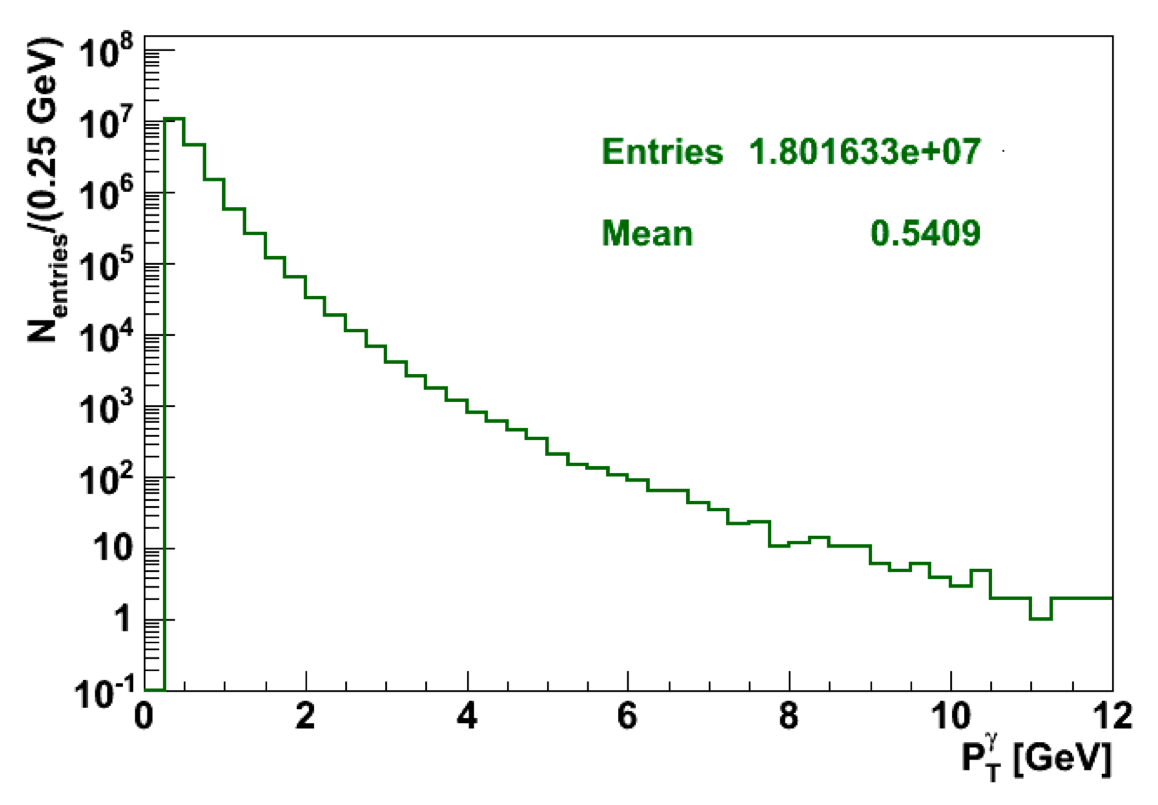
\includegraphics[width=.45\textwidth]{ptMC.png}
\caption{Transverse momentum spectrum of converted photons in minimum
  bias MC events at $\sqrt{s}=900\GeV$.}
\label{ptMC}
\end{figure}

The present analysis makes use of the algorithm described in~\cite{nancy}.
It allows the reconstruction of low-$p_T$ photons ($\geq 0.4\GeV$)
without any request of ECAL match. The main signature for the
conversion identification is the reconstruction of two opposite
charged tracks with tangent direction at the point where they form a
detached vertex. The vertex fit is performed with the \emph{Kinematic
  Constraint Vertex Fitter}.





\section{Photon Conversion Reconstruction}
\label{standard}


Up to 70\% of photons traversing the Tracker material converts into  $e^+ e^-$ pairs.
In the Minimum Bias events collected during the  first phase of CMS data taking, photons, mainly coming from
$\pi^0$ decays, are expected to have a very soft spectrum. The electron pairs from conversions are very unlikely to
reach the Electromagnetic Calorimeter (ECAL) and the ECAL cluster-driven track and seed finding method~\cite{NOTE2006005, EGM-10-005}
cannot be applied. The development of the iterative tracking described in~\cite{TRK-10-001}
largely extended the capability of reconstructing low-\pt tracks and displaced vertices.
Furthermore, for the work presented in this Analysis Summary, additional seeding steps were introduced as described in Sec.~\ref{sec:newSeedingSteps}
and exploited here to improve the identification of conversions at large radii.
The tracker-only conversion reconstruction was already partially commissioned with limited statistics
during the LHC runs at $\sqrt{s}=900\GeV$ data~\cite{TRK-10-001}.


The conversion information can be obtained by the reconstruction of the e+ and e? tracks of the
	conversion. Two methods are used and compared, ECAL-seeded conversion method and combined conversion method. One method only uses the conversion ECAL-seeded tracks and the 	other takes into account conversion track pairs reconstructed from a combination of standard 	tracks, Gaussian sum filter (Gsf) tracks and conversion ECAL-seeded tracks. We first check various kinematical distributions of selected photons in ECAL-seeded conversion method, followed by combined conversion method.


Both methods (ECAL-seeded and combined) 	fit two oppositely charged tracks to a common vertex with the constraint that the two tracks 	are parallel at the vertex, in both the transverse and longitudinal planes. The methods differ 	mainly in the preselection of the track pairs.

%\subsection{Selection and results}                                                                                                                                                                


Photon conversions are characterized by a pair of
oppositely charged secondary tracks, originating from the photon vertex with an
invariant mass consistent with zero,  which are therefore parallel
to each other at production vertex. The electron-positron pair, then,
opens only in the transverse plane because of the solenoidal magnetic field.



In this analysis we use the tracker-driven conversion reconstruction,
already described in~\cite{TRK-10-001}, in~\cite{trk10001} and in~\cite{TRK-10-003}. We
summarize the method here mentioning the further requirements needed to  
specialize the tracker conversion reconstruction to the $\chi_c$
case. The algorithm relies on the capability of iterative tracking,
discussed in~\cite{TRK-10-001}, to efficiently reconstruct low-\pt and
displaced tracks, as the ones coming from a photon conversion.

Opposite-sign track pairs are firstly required to satisfy basic
quality criteria, i.e. have more than four hits and a normalised
$\chi^2$ less than 10. Then
the tracker-only conversion finding exploits the conversion pair
signature to distinguish genuine pairs from fake pairs.
Tracks are required to have positive charge-signed transverse impact
parameter (the primary vertex lies outside the track trajectory helix)
and the distance of minimum approach in the $xy$ plane, $d_m$, between $-0.25\cm$
and $1\cm$ where $d_m$ is
%defined as $d_{O_1-O_2} - (R_1 - R_2)$ where
%$d_{O_1-O_2}$ is the distance between the centres of the two track
%circles in the transverse plane and $R_1$ and $R_2$ are the two
%circles radii.
the distance between the two points of tangent approach in the
transverse plane for the helices of the two tracks.




Track pairs surviving the selection are then fitted to a common
3D-constrained kinematic vertex fitter. The 3D constraints imposes the
tracks to be parallel in both the transverse and longitudinal planes.
The pair is retained if the fit converges and its $\chi^2$ probability
is greater than $5\times10^{-4}$.



Conversion vertices are reconstructed with an excellent precision:
the angular resolution is about $1{\rm mrad}$ while the radial resolution varies from about~$0.2\cm$ to about~$0.5\cm$, primarily
as a function of pseudo-rapidity.
In Fig.~\ref{fig:convXY} the position of conversion vertices reconstructed in data is shown in the $(x,y)$ plane:
in Fig.~\ref{subfig:convXY_a} the structure at the very centre is the Pixel detector,
surrounded by the shell and rails supporting the Pixel detector, four layers of the Inner Tracker and the first layer of the Outer Tracker.
When restricting the $(x,y)$ view to $\pm 12\cm$, Fig.~\ref{subfig:convXY_c}, the beam pipe is clearly visible, off-centered with respect to
the Pixel detector. More details on the features visible on the ``radiographies'' are given in Sec.~\ref{sec:mat}.

The  $(z, R)$  view of conversion vertices reconstructed in data is finally shown in Fig.~\ref{fig:convRZ};  the less populated
areas  around $|\eta|\sim1.2$, also present in simulation, correspond to transition regions between the Tracker
barrel and endcap sub-components for which the additional track seeding
iterations described in Sec.~\ref{sec:newSeedingSteps} have not been optimized and the conversion reconstruction efficiency is smaller.

\begin{figure}[h!]
  \begin{center}
   \vspace{-0.6cm}
   \subfigure[]{
   \label{subfig:convXY_a}
    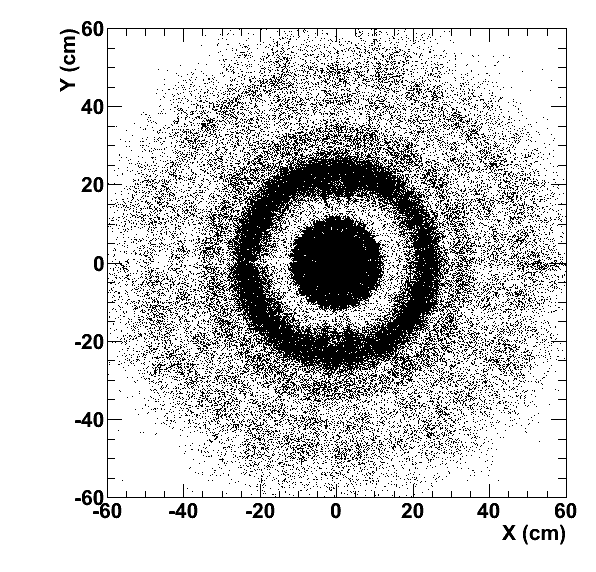
\includegraphics[width=0.40\textwidth]{fig/conversions/ptCut/data_xy.png}}
   \subfigure[]{
   \label{subfig:convXY_b}
    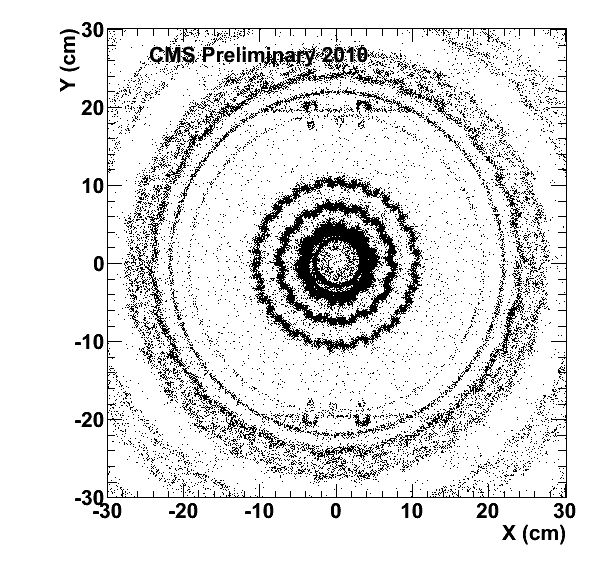
\includegraphics[width=0.40\textwidth]{fig/conversions/ptCut/data_xy_zoom.png}}
   \subfigure[]{
   \label{subfig:convXY_c}
    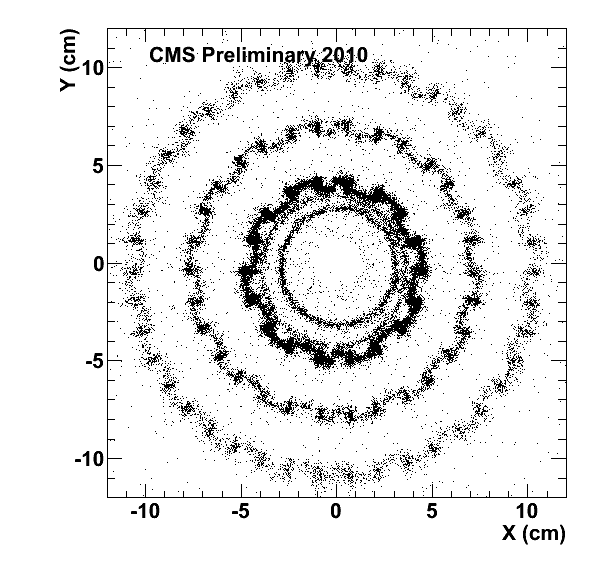
\includegraphics[width=0.40\textwidth]{fig/conversions/ptCut/data_xy_pixel_eta.png}}
    \caption{Conversion vertices in data in the $(x,y)$ plane for $|z|<26\cm$; zoom increases from (a) to (c).}
    \label{fig:convXY}
  \end{center}
\end{figure}

\begin{figure}[h!]
  \begin{center}
     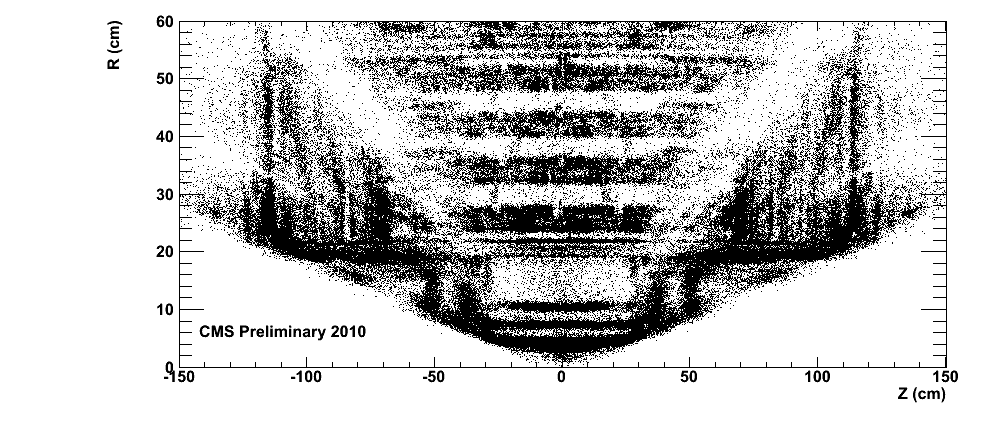
\includegraphics[width=15cm,height=5.5cm]{fig/conversions/ptCut/data_rz.png}
      \caption{Conversion vertices in data the $(z,R)$ plane.}
    \label{fig:convRZ}
  \end{center}
\end{figure}


\begin{figure}[!hbtp]
\centering
\subfigure[]{
\label{subfig:TIBL1Int_LocView_sim}
\includegraphics[width=.32\textwidth]{fig/L1_INT_sim_mod.png}}
\subfigure[]{
\label{subfig:TIBL1Int_LocView_mc}
\includegraphics[width=.32\textwidth]{fig/L1_INT_mc_mod.png}}
\subfigure[]{
\label{subfig:TIBL1Int_LocView_data}
\includegraphics[width=.32\textwidth]{fig/L1_INT_data_mod.png}}
\caption{Nuclear interaction local view of the $x_{\rm local}$ vs. $z_{\rm local}$ projection related to the Inner Tracker Layer 1, internal part: \subref{subfig:TIBL1Int_LocView_sim}~simulation\
 truth; \subref{subfig:TIBL1Int_LocView_mc}~simulation reconstructed; \subref{subfig:TIBL1Int_LocView_data}~data.}
\label{fig:TIBL1Int_LocView}
\end{figure}

As an example of this technique, the local transverse view, $x_{\rm local}$ vs. $z_{\rm local}$ with respect to the R$\phi$ module, of the Inner Strip Tracker Layer 1, internal, is shown in Fig.\
~\ref{fig:TIBL1Int_LocView} for nuclear interaction vertices. Each plot features the single module local view replicated three times, with the appropriate relative geometry, to mock-up a portion\
 of the structure.
The data based plot of Fig.~\ref{fig:TIBL1Int_LocView}~\subref{subfig:TIBL1Int_LocView_data} shows the structures expected in the simulation but affected by the smearing due to misalignment and \
unavoidable irregularities of the passive structures.




\section{Tracking Improvement}
\label{singleleg}


The standard CMS tracking is made of six iterative steps, numbered
from 0 to 5, designed to obtain high efficiency and low fake rate for
tracks coming either from the primary vertex or from displaced decay
vertices while maintaining the overall computing time within the
requirements of CMS offline reconstruction centre.
Because of this constraint, the standard implementation is not optimal
to reconstruct with high efficiency tracks from photon conversions and
nuclear interactions since the cuts applied in the standard
reconstruction are too tight for these processes. In fact, those
tracks have usually very low momentum and, especially for displaced
vertices at large radii, they do not point  back to the primary
vertex; therefore, they could be reconstructed only with very relaxed
cuts that would result into unacceptably large computing time during
the pattern recognition.

For the purpose of the present study, two additional dedicated
tracking steps are added to the track reconstruction sequence.
These were specifically designed to increase the number of
reconstructed conversion vertices in the barrel region,
but they have been found to be very useful for nuclear interaction as
well. A first additional step (step 6) is seeded from triplets of hits
in the Pixel barrel and/or in the Strip Tracker Inner barrel
detectors; a second additional step (step 7) is seeded from hit-pairs
in the Strip Tracker barrel detectors and/or in the Strip Tracker Inner disks.
The seed trajectories are required
%to originate from a region of radius $25\cm$ and longitudinal half length of $0.5\cm$ and are required                                                                                            
to have a minimum transverse momentum of $0.1$ and $0.2\GeVc$ for the
step 6 and 7, respectively. The resulting large number of seeds is
reduced by selecting topologies compatible with a photon conversion
pair: the total charge has to be zero,
the azimuthal angle difference less than $1.5$ radians, the difference
in the cotangent of the polar angle less than $0.25$ radians, and the
differences of the radial and longitudinal coordinates of the
innermost hit have to be less then $5\cm$.
The pattern recognition is then performed allowing for at most one
lost hit and requiring at least three hits. Finally the standard track
fit provides the best estimate of the track parameters.

The impact of the additional steps to the reconstruction of conversion
and nuclear interaction vertices can be seen on Fig.~\ref{fig:matItTk}
showing the contribution of the different steps to the vertices
reconstruction, as estimated by the simulation.
Step 7 increases by more than a factor two the number of conversions
outside the Pixel detector region and contributes significantly to nuclear
interaction vertices at all radii; step 6 mainly helps finding
conversions in the second and third Pixel detector layers. Further details
about the reconstruction of conversions and nuclear interactions will
be given in the following sections.
\begin{figure}[!hbtp]
\centering
\subfigure[]{
\label{subfig:convItTk}
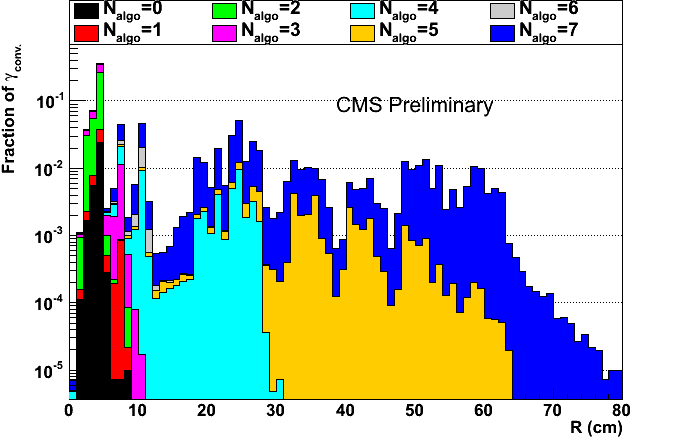
\includegraphics[width=.7\textwidth]{fig/r_algo_BasicCutsJuly12.png}}
\subfigure[]{
\label{subfig:nuclItTk}
\includegraphics[width=.7\textwidth]{fig/r_algo_2010-06-04_NI.png}}
\caption{Fraction of reconstructed vertices as a function of the radius of the vertex
for conversions~\subref{subfig:convItTk} and nuclear
interactions~\subref{subfig:nuclItTk}, for  $|\eta|<1.4$, as estimated
from simulation. The different colors correspond to the largest
iterative step needed to reconstruct the tracks at the vertex.}
\label{fig:matItTk}
\end{figure}


\include{otherseed}

%\thispagestyle{empty}
\section{Conclusions}
\label{conclusions}


%\newpage
\section*{References}

\begin{thebibliography}{99}
\bibitem{cms}
  Adolphi R et al. [CMS Collaboration] 2008 The CMS experiment at the CERN LHC
  {\em JINST} {\bf 3} S08004 
\bibitem{TkTDR} CMS Collaboration 1998 The Tracker System Project Technical Design Report
  {\em CERN-LHCC} 98-6
\bibitem{TkTDRadd} CMS Collaboration 2000 Addendum to the CMS Tracker TDR {\em
   CERN-LHCC} 2000-16
\bibitem{trackreco} CMS Collaboration 2010 Tracking and Vertexing Results from First Collisions
{\em CMS-PAS} TRK-10-001
\bibitem{cmssw} CMS Collaboration 2006 CMS Physics Technical Design
    Report Detector Performance and Software {\em
      CERN-LHCC} 2006-001
\bibitem{posterConv} Giordano D and Sguazzoni G [CMS
  Collaboration] 2012 An innovative seeding technique for photon conversion
  reconstruction at CMS {\em these proceedings}
\bibitem{kdtree} Bentley J L 1975 Multidimensional binary search
    trees used for associative searching {\em Commun. ACM} {\bf 18} 9 (Sep. 1975) 509-517 
\bibitem{parallel} Hauth T, Innocente V and Piparo D [CMS
  Collaboration] 2012 Development and Evaluation of Vectorised and
    Multi-Core Event Reconstruction Algorithms within the CMS Software
    Framework {\em these proceedings}
\end{thebibliography}


\end{document}
